% !TeX root = ../FC19_Slides.tex
% \tableofcontents
% ---------------------------------------------------------%

\section{Introduction}

\subsection{Monero}
\begin{frame}{Monero}\label{sec:monero}
	\begin{itemize}
		\item Public nature of Bitcoin TX history prevents meaningful level of anonymity
		\item Monero (based on CryptoNote, \cite{van_saberhagen_cryptonote_2013}) addresses this with the following methods:
		\begin{itemize}[<+-|alert@+>]
			\item Stealth Addresses (hide recipient addr.) $\to$ unlinkability
			\item \alert<4->{Ring Signatures (obfuscate spent TXO) $\to$ untraceability}
			\item Confidential Transactions (hide amounts) $\to$ fungibility
		\end{itemize} 
	\end{itemize}
\end{frame}

\subsection{Ring Signatures}
\begin{frame}{Ring Signatures \& Traceability}
	\vspace*{-10pt}
	\begin{itemize}[<+->]
		\item Each TX input references:
		\begin{itemize}
			\item Bitcoin: Output from older TX (TXO)
			\item Monero: Non-empty set of TXOs (a ring)
		\end{itemize}
		\item One ringmember is real, the others are decoys (mixins)
		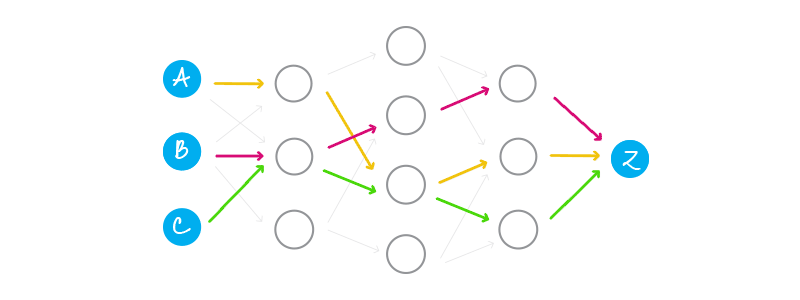
\includegraphics[width=0.9\textwidth]{./img/slides/cn-44.png}
{		\hspace*{90pt}\scriptsize Source: \url{https://cryptonote.org/inside/}}
		\item Decoys are sampled from set of eligible outputs
	\end{itemize}
\end{frame}

\subsection{Traceability Methods}
\begin{frame}{Known Traceability Methods}
	\begin{itemize}[<+-|alert@+>]
		\item Zero Mixin Removal (ZMR)
		\begin{itemize}
			\item remove known spent outputs from rings
		\end{itemize}
		\item Intersection removal (IR)
		\begin{itemize}
			\item generalized ZMR; ``closed set attack''
		\end{itemize}
		\item Output Merging Heuristic (OMH)
		\begin{itemize}
			\item outputs were split up into denominations; if two outputs from a single TX are redeemed in another TX, assume that those inputs are real
		\end{itemize}
		\item Guess Newest Heuristic (GNH)
		\begin{itemize}
			\item temporal distribution of mixins and real spending behavior didn't match - most recent input often the real one
		\end{itemize}
	\end{itemize}
\end{frame}

%\subsection{Previous Results}
% \begin{frame}{Traceability Analysis}
% 	\cite{kumar_traceability_2017} and \cite{moser_empirical_2018} found:
% 	\begin{itemize}[<+->]
% 		\item Iteratively removing known spent outputs from rings allows identification of new spent outputs
% 		\begin{itemize}
% 			\item $\to$ identified majority of real spent outputs
% 		\end{itemize}
% 		\item TX outputs were partitioned into denominations (7 $\to$ 5 + 2)
% 		\begin{itemize}
% 			\item $\to$ guessing real inputs mostly correct
% 		\end{itemize}
% 		\item Temporal distribution of decoys and spent outputs don't match
% 		\begin{itemize}
% 			\item $\to$ Educated guessing based on output-age effective 
% 		\end{itemize}
% 		\item Transaction protocol has been updated since 
% 	\end{itemize}
% \end{frame}




\begin{frame}{Improvements to the protocol}
	\begin{itemize}
		\item ZMR works like a chain reaction from an initial set of inputs without decoys.
		\begin{itemize}
			\item Since 2016, the mandatory minimum ringsize has been increased
			\item Minimum ringsizes + RingCT TX were effective
			\item Ringsize $\equiv 11$ since last update
		\end{itemize}
		\item Mixin sampling has been improved with different approaches
		\begin{itemize}
			\item Triangular distribution
			\item Recent zone: Force 25-50\% recent outputs
			\item Gamma distribution: Distribution based on empirical analysis
		\end{itemize}
	\end{itemize}
\end{frame}

\section{Our contribution}
\subsection{Overview}
\begin{frame}{Contribution of this work}
	\begin{itemize}
		\item Reevaluation of existing methods
		\begin{itemize}
			\item Previous studies published shortly after introduction of RingCT
			\item Changes to mixin sampling and ringsize in 09/2017 and 04/2018.
		\end{itemize}
		\item Quantification of impact due to recent (Spring 2018) Monero hardforks
		\begin{itemize}
			\item Monero Original: Continuation of Monero v6 (ASIC compatible)
			\item MoneroV: Fork with some changes to emission curve
		\end{itemize}
	\end{itemize}
\end{frame}

\subsection{Cross Chain Analysis (CCA)}
\begin{frame}{Currency hardforks}
	\begin{itemize}
		\item A cryptocurrency can be forked, resulting in two currencies with a shared TX history
		\begin{center}
			% !TeX root = ../../CI-Poster.tex
\begin{tikzpicture}[scale=0.8%, every node/.style={transform shape}
    , every node/.style={transform shape,XMRColor, ultra thick, shape border rotate = 180}
    , box/.style={minimum height = 30pt, minimum width = 30pt}
    , arr/.style={single arrow, minimum width = 30pt, minimum height = 40pt, anchor=tip}
    ]
\node[box] (last) at (-2,0){0};% top color=vir6, bottom color=vir8,
\node[arr] (last) at (last.east) {1};%\node[arr] (last) at (last.east) {2};
\node[arr, inner sep=20pt] (last) at (last.east) {\ldots};
\node[arr] (f1) at (last.east) {$n$};
% Fork 1 
\node[arr,rotate=22] (last) at (f1.before tail){$n+1$};
    \node[arr,xshift = 0.5mm] (last) at (last.east) {$n+2$};
    \node[arr, inner sep=20pt] (last) at (last.east) {\ldots};
% Fork 2
\node[arr, XMVColor, rotate = -22] (last) at (f1.after tail){$n+1$};
    \node[arr,XMVColor,xshift = 0.5mm] (last) at (last.east) {$n+2$};
    % \node[arr,XMVColor] (last) at (last.east) {$n+3$};
    \node[arr,XMVColor] (last) at (last.east) {$n+4$};
    \node[arr,XMVColor, inner sep=20pt] (last) at (last.east) {\ldots};
\end{tikzpicture}
		\end{center}
		\item Pre-fork funds can be spent on both chains
		\item Monero prevents double spends with \emph{key images} (unique identifier derived from spent output)
		\item<2-> If two rings on separate branches share a key image, they spend the same output.
	\end{itemize}
\end{frame}

% \begin{frame}{Cross Chain (Fork) Analysis}
% \begin{itemize}[<+->]
% 	% \item Bitcoin \& Bitcoin Cash:
% 	% \begin{itemize}
% 	% 	\item Multiple Input Heuristic employed by GraphSense
% 	% 	\item If pre-fork funds are spent, addresses could be clustered on both post-fork branches
% 	% \end{itemize}
% 	% \item Monero:
% 	% \begin{itemize}
% 		\item Double spends are prevented with \emph{key images}
% 		\item Key image is derived from spent output and may occur at most once on the TX record
% 		\item Method to derive key image must be identical on all branches
% 		\item If two rings on two branches have the same key image, they spend the same TXO. 
% 	% \end{itemize}
% \end{itemize}
% \end{frame}



\subsection{Dataset}
\begin{frame}{Dataset \& Method}
	\begin{enumerate}
		\item Exported Monero (XMR), MoneroV (XMV) and Monero Original (XMO) blockchain up to Aug. 31$^\text{th}$, 2018.
		\item Employed Zero Mixin Removal \& Intersection Removal
		\item Added fork data and applied cross chain analysis (+ZMR/IR)
		\item Applied heuristics from \cite{kumar_traceability_2017} and \cite{moser_empirical_2018}:
		\begin{itemize}
			\item Guess Newest Heuristic
			\item Output Merging Heuristic
		\end{itemize}
		\item Evaluated accuracy with ground truth (where possible) with results from steps 3 (OMH see paper).
	\end{enumerate}
\end{frame}

\begingroup
\small
\section{Results}
\subsection{Results}
\begin{frame}{Traced Inputs}
	\def\imgFile{./img/slides/linked.tex}
	\input{\imgFile}
\end{frame}
\begin{frame}{Guess Newest Heuristic}
	\def\imgFile{./img/slides/guess_newest.tex}
	\input{\imgFile}
\end{frame}
\endgroup

\normalsize
\subsection{Summary}
\begin{frame}{Summary}
	\begin{itemize}[<+-|alert@+>]
		\item Nowadays, most Monero TXs are untraceable with known passive attack vectors
		\item Guess Newest Heuristic does not work with current mixin sampling technique
		\item Impact from Cross Chain Analysis not very large
		\begin{enumerate}
			\item Forks so far didn't have a lot of traction (maybe disputes over ASICs change that)
			\item Mandatory ringsize of 7 enough to prevent chain reactions (11 is even better)
		\end{enumerate}
	\end{itemize}
	\uncover<5->{Data \& source available:\hspace*{20mm}\qrcode[height=18mm]{https://github.com/oerpli/MONitERO}}
\end{frame}


\subsection{References}
\begin{frame}{References}
    \bibliographystyle{apalike-refs}
    \bibliography{cryptoSlides}
\end{frame}
\backupbegin
\appendix




% And your backup slides here
% \subsection{Cryptocurrencies}
% \begin{frame}{Cryptocurrencies}
	% 	\begin{itemize}
		% 	\item \cite{nakamoto_bitcoin:_2008}	laid the foundation of modern cryptocurrencies (scheme for trusted decentralized transactions)	
		% 	\item Transactions have inputs (references to previous outputs) and outputs
		% 	\item Each output is issued to address of a user (public key)
		% 	\item Recipient can spend outputs with private key
	% 	\end{itemize}
% \end{frame}

% \begin{frame}{Blockchain}
% 	\resizebox{\textwidth}{!}{% !TeX root = ../CI-Thesis.tex
\begin{tikzpicture}[
	,	scale=1.0
	,	node distance=4mm,
	,	font=\ttfamily,
	,	BlockTitle/.style={font=\fontsize{12}{12}\color{black!80}\ttfamily}
	,	TXHeader/.style={below=of T.west,anchor=north west, yshift = -3.5mm}
] 
\def\dist{5}

\node[BlockTitle] (Bt) at ($(\dist*0,0)$) {Block 0 };
\node[below=of Bt.west,anchor=north west] (Hash0) {Hash: \href{https://blockchain.info/de/block/000000000019d6689c085ae165831e934ff763ae46a2a6c172b3f1b60a8ce26f}{000019d668}};
\node[below=of Hash0.west,anchor=north west] (Prev0) {Prev: 0000000000};
\node[below=of Prev0.west,anchor=north west] (T) { Nonce: 208323689};
%\node[TX, below=of T.west,anchor=north west,opacity=0] (T) { TX1: \ 0af121280a };
\node[below=of T.west,anchor=north west] (T) { Time: 2009-01-03};
\node[below=of T.west,anchor=north west] (T) { Merkle R.: 4a5e3};


\node[TXHeader] (TXt) {TX Merkle Tree};

\node[TX,txColorLight, below=of TXt.west,anchor=north west] (TXs) { TX0: \ \href{https://blockchain.info/de/tx/4a5e1e4baab89f3a32518a88c31bc87f618f76673e2cc77ab2127b7afdeda33b}{4a5e321e4b}};

\begin{scope}[on background layer]
	\node[Block,fit={(Bt) (T)}] (B1) {};
	\node[BlockD,fit={(Prev0) (T)}] (B1h) {};
	\node[BlockD,draw=black, fill=none, inner sep = 1pt, very thick, dotted, fit={(Prev0) (T)}] (B1H) {};
	\node[TX,fit={(TXt)(TXs)}] (TXb2) {};
	\node[TX, draw=black, fill=none, thick, inner sep = 1pt, dashed, fit={(TXb2)}] (MRH) {};
\end{scope}
\path[thick, dashed, black,-latex]($(T.east)-(0.1,0)$) edge[out = 0, in = 0] (MRH.east);

\node[BlockTitle] (Bt) at ($(\dist*1,0)$) {Block 1 };
\node[below=of Bt.west,anchor=north west] (Hash1) {Hash: \href{https://blockchain.info/de/block/00000000839a8e6886ab5951d76f411475428afc90947ee320161bbf18eb6048}{0000839a8e}};
\node[below=of Hash1.west,anchor=north west] (Prev1) {Prev: 000019d668};
\node[below=of Prev1.west,anchor=north west] (T) { Nonce: 257339468};
%\node[TX, below=of T.west,anchor=north west] (T) { TX1: \ 0ab112023a };
\node[below=of T.west,anchor=north west] (T) { Time: 2009-01-09 };
\node[below=of T.west,anchor=north west] (T) { Merkle R.: 0e3e2};


\node[TXHeader] (TXt) {TX Merkle Tree};
\node[TX,txColorLight, below=of TXt.west,anchor=north west] (TXs) { TX0: \ \href{https://blockchain.info/de/tx/0e3e2357e806b6cdb1f70b54c3a3a17b6714ee1f0e68bebb44a74b1efd512098}{0e3e2357e8}};

\begin{scope}[on background layer]
	\node[Block,fit={(Bt) (T)}] (B1) {};
	\node[BlockD,fit={(Prev1) (T)}] (B1h) {};
	\path[thick, dashed, black,-latex, dotted]($(Prev1.west)+(0.1,0)$) edge[out=180, in = 0] (B1H.east);
	\node[BlockD,draw=black, fill=none, inner sep = 1pt, very thick, dotted, fit={(Prev1) (T)}] (B1H) {};
	\node[TX,fit={(TXt)(TXs)}] (TXb2) {};
	\node[TX, draw=black, fill=none, thick, inner sep = 1pt, dashed, fit={(TXb2)}] (MRH) {};
\end{scope}
\path[thick, dashed, black,-latex]($(T.east)-(0.1,0)$) edge[out = 0, in = 0] (MRH.east);

% \draw[ultra thick,-latex] (Prev1.west)--(Hash0.east);

\node[BlockTitle] (Bt) at ($(\dist*2,0)$) {Block 2 };
\node[below=of Bt.west,anchor=north west] (Hash2) {Hash: \href{https://blockchain.info/de/block/00000000d1145790a8694403d4063f323d499e655c83426834d4ce2f8dd4a2ee}{0000d11457}};
\node[below=of Hash2.west,anchor=north west] (Prev2) {Prev: 0000839a8e};
\node[below=of Prev2.west,anchor=north west] (T) { Nonce: 188941879};
\node[below=of T.west,anchor=north west] (T) { Time:  2009-01-12 };
\node[below=of T.west,anchor=north west] (T) { Merkle R.: f4f8a};


\node[TXHeader] (TXt) {TX Merkle Tree};
\node[TX,txColorLight, below=of TXt.west,anchor=north west] (TXs) { TX0: \ \href{https://blockchain.info/de/tx/b1fea52486ce0c62bb442b530a3f0132b826c74e473d1f2c220bfa78111c5082}{b1fea52486}};
\node[TX,txColorLight, below=of TXs.west,anchor=north west] (TXs) { TX1: \ \href{https://blockchain.info/de/tx/f4184fc596403b9d638783cf57adfe4c75c605f6356fbc91338530e9831e9e16}{f4184fc596}};

\begin{scope}[on background layer]
	\node[Block,fit={(Bt) (T)}] (B1) {};
	\node[BlockD,fit={(Prev2) (T)}] (B1h) {};
	\path[thick, dashed, black,-latex, dotted]($(Prev2.west)+(0.1,0)$) edge[out=180, in = 0] (B1H.east);
	\node[TX,fit={(TXt)(TXs)}] (TXb2) {};
	\node[TX, draw=black, fill=none, thick, inner sep = 1pt, dashed, fit={(TXb2)}] (MRH) {};
\end{scope}
\path[thick, dashed, black,-latex]($(T.east)-(0.1,0)$) edge[out = 0, in = 0] (MRH.east);

% \draw[ultra thick,-latex] (Prev2.west)--(Hash1.east);

\end{tikzpicture} }
% \end{frame}

% \begin{frame}{Transaction}
	% 	\resizebox{\textwidth}{!}{% !TeX root = ../CI-Thesis.tex
\begin{tikzpicture}[
	,	scale=1.0
	,	node distance=4mm,
	,	font=\ttfamily\bfseries,
	,	BlockTitle/.style={font=\fontsize{12}{12}\color{black!80}\ttfamily\bfseries}
	,	TxTitle/.style={font=\fontsize{12}{12}\color{white}\ttfamily\bfseries}
	,	-latex
] 
\def\dist{6}

% https://webbtc.com/tx/a1075db55d416d3ca199f55b6084e2115b9345e16c5cf302fc80e9d5fbf5d48d.json

\node[TxTitle] (BT) at ($(\dist*0,0)$) {TX Hash:\ \href{https://blockchain.info/de/tx/be83f7760b5f1a91ebe8666e719cd0b7e8c66d1ceb9d151c401f41934b1cebe9}{be83f7760b5f1a91}};
\node[below=of BT.west,anchor=north west] (Hash0) {Version no:\quad1};
\node[below=of Hash0.west,anchor=north west] (Hash0) {\#Inputs:\qquad\ 2};
\node[below=of Hash0.west,anchor=north west] (numOut) {\#Outputs:\quad\ \ 2};

\node[below=of numOut.west,anchor=north west] (H1) {TX Hash/Index:\ \href{https://blockchain.info/de/tx/ba7521ec534fb14f8da39dc3460281e8db98aa4d016226f252b301616f0721e1}{ba7521ec}/2};
\node[below=of H1.west,anchor=north west] (Sig1) {Signature: 3045022100c\ldots};

\node[below=of Sig1.west,anchor=north west, yshift=-2mm] (H2) {TX Hash/Index:\ \href{https://blockchain.info/de/tx/888e046478c9b004c4f45e24851052989ebdf666b61369524a9ca69a1bc5aa91}{888e0464}/1};
\node[below=of H2.west,anchor=north west] (Sig2) {Signature: 30440220244\ldots};


\node[right=of BT.south east,anchor=north west,yshift=-0.6mm, xshift=3mm] (Outs) {Outputs:};
\node[below=of Outs.west,anchor=north west] (i1) {0:};
\node[right=of i1.north east,anchor=north west] (O1) {\ \ \ \ \ Value: 1.99713455};
\node[below=of i1.west,anchor=north west] (O1) {Recipient addr: \href{https://blockchain.info/address/126uLE1GDFxjjV5enHZzSGHJHiupH67FmA}{126uLE1GDFxj}};
\node[below=of O1.west,anchor=north west] (O1) {scriptPubKey: \ldots{}OP\_CHECKSIG};
\node[below=of O1.west,anchor=north west, yshift=-2mm] (i2) {1:};
\node[right=of i2.north east,anchor=north west] (O2) {\ \ \ \ \ Value: 6.00255800};
\node[below=of i2.west,anchor=north west] (O2) {Recipient addr:  \href{https://blockchain.info/address/16jaR3vF4TH3ZdHJeRfVW8a5VYH2NbvbSB}{16jaR3vF4TH3}};
\node[below=of O2.west,anchor=north west] (O2) {scriptPubKey: \ldots{}OP\_CHECKSIG};

\node[opacity=0, right=of O2.east, xshift=-6mm, yshift=-2mm](Stretch){ };
\begin{scope}[on background layer]
	\node[TX,fit={(BT) (Sig2) (Stretch)}] (B1) {};
	\node[BlockD,fit={(H1) (Sig1)}] (B1h) {};
	\node[BlockD,fit={(H2) (Sig2)}] (B1h) {};
	\node[Block,fit={(Outs) (O2)}] (B1h) {};

	\node[BlockD,fit={(i1) (O1)}] (B1h) {};
	\node[BlockD,fit={(i2) (O2)}] (B1h) {};

	\node[outIndex, fit={(i1)}, xshift=-0.55mm, yshift=0.55mm] (B1h) {};
	\node[outIndex, fit={(i2)}, xshift=-0.55mm, yshift=0.55mm] (B1h) {};
\end{scope}

\end{tikzpicture} }
% \end{frame}

% \begin{frame}{Bitcoin analytics}
	% 	\begin{itemize}
		% 		\item Analysis techniques impeded privacy of Bitcoin
		% 		\item Sets of addresses belonging to a user can often be identified 
		% 		\begin{itemize}
			% 			\item Multi Input Heuristic
			% 			\item Change Heuristics
		% 		\end{itemize}
		% 		\item Simplified transaction graph allows further analysis
	% 	\end{itemize}
% \end{frame}


\begin{frame}{Zero Mixin Removal \& Intersection Removal}
	\resizebox{\textwidth}{!}{% !TeX root = ../../CI-Slides.tex
\begin{tikzpicture}[scale=1.0, -{Latex[length=3mm, width=1.5mm]}
    ,    remEdge/.style={thick, dashed, virNodeDark=1.0} 
    ,    sureEdge/.style={thick, virNodeDark=0.7} 
    ,    spentEdge/.style={thick, dashed, virNodeDark=0.7}] 
\coordinate (C1) at (2,2);

\begin{scope}[xshift=-5.0cm]
    \node[virNode=0.45] (X1) at (-1,0.9){O1}; 
    \node[virNode=0.60] (X2) at (-1,0){O2}; 
    \node[virNode=0.75] (X3) at (-1,-0.9){O3}; 
    \node[virNode=0.90] (X4) at (-1,-0.9*2){O4}; 
    \node[virNode=0.0,text=white] (Y1) at (1,0.9){R1};
    \node[virNode=0.05,text=white] (Y2) at (1,0){R2};
    \node[virNode=0.1,text=white] (Y3) at (1,-0.9){R3};
    \node[virNode=0.15,text=white] (Y4) at (1,-0.9*2){R4};
   
    \path[thick, nodeBlack](X1) edge[] (Y1);
    \path[thick, nodeBlack](X1) edge[] (Y2);
    \path[thick, nodeBlack](X2) edge[] (Y2);
    \path[thick, nodeBlack](X3) edge[] (Y2);
    \path[thick, nodeBlack](X3) edge[] (Y3);
    \path[thick, nodeBlack](X3) edge[] (Y4);
    \path[thick, nodeBlack](X4) edge[] (Y3);
    \path[thick, nodeBlack](X4) edge[] (Y4);
\end{scope}
\uncover<2->{
\begin{scope}[xshift=0.0cm]
    \node[virNode=0.45] (X1) at (-1,0.9){O1}; 
    \node[virNode=0.60] (X2) at (-1,0){O2}; 
    \node[virNode=0.75] (X3) at (-1,-0.9){O3}; 
    \node[virNode=0.90] (X4) at (-1,-0.9*2){O4}; 
    \node[virNode=0.0,text=white] (Y1) at (1,0.9){R1};
    \node[virNode=0.05,text=white] (Y2) at (1,0){R2};
    \node[virNode=0.1,text=white] (Y3) at (1,-0.9){R3};
    \node[virNode=0.15,text=white] (Y4) at (1,-0.9*2){R4};
    
    \path[sureEdge](X1) edge[] (Y1);
\uncover<4->{
    \path[remEdge](X1) edge[] (Y2);
    \path[remEdge](X3) edge[] (Y2);
}
\uncover<5->{
    \path[sureEdge](X2) edge[] (Y2);
}
\uncover<3->{
    \path[spentEdge](X3) edge[] (Y3);
    \path[spentEdge](X3) edge[] (Y4);
    \path[spentEdge](X4) edge[] (Y3);
    \path[spentEdge](X4) edge[] (Y4);
}
\end{scope}
}
\uncover<5->{
\begin{scope}[xshift=5.0cm]
    \node[virNode=0.45] (X1) at (-1,0.9){O1}; 
    \node[virNode=0.60] (X2) at (-1,0){O2}; 
    \node[virNode=0.75] (X3) at (-1,-0.9){O3}; 
    \node[virNode=0.90] (X4) at (-1,-0.9*2){O4}; 
    \node[virNode=0.0,text=white] (Y1) at (1,0.9){R1};
    \node[virNode=0.05,text=white] (Y2) at (1,0){R2};
    \node[virNode=0.1,text=white] (Y3) at (1,-0.9){R3};
    \node[virNode=0.15,text=white] (Y4) at (1,-0.9*2){R4};

    \path[sureEdge](X1) edge[] (Y1);
    \path[sureEdge](X2) edge[] (Y2);
    \path[spentEdge](X3) edge[] (Y3);
    \path[spentEdge](X3) edge[] (Y4);
    \path[spentEdge](X4) edge[] (Y3);
    \path[spentEdge](X4) edge[] (Y4);
\end{scope}
}
\end{tikzpicture} }
	\begin{itemize}
		\item Outputs O1-O4 are referenced in rings R1-R4
		\item<2-> R1 only references O1 $\implies$ must be the real input
		\item<3-> $I = \{R3,R4\}$ reference $O=\{O3,O4\}$  \\
		\qquad	$|I| = |O|$ $\implies$ O3 \& O4 spent in R3 \& R4
		\item<4-> $R2$ only has one non-mixin reference remaining.
	\end{itemize}
\end{frame}

\begin{frame}{Output Merging Heuristic (OMH)}
	\begin{itemize}
		\item Output merging mostly due to denomination splitting:
		\begin{itemize}
			\item Initially, amounts were disclosed on blockchain
			\item Ring signatures required multiple outputs with identical amounts
			\item Outputs were partitioned to facilitate this (7 $\to$ 5 + 2)
		\end{itemize}
	\end{itemize}
	\uncover<2->{
		\resizebox{\textwidth}{!}{% !TeX root = ../../CI-Slides.tex
\begin{tikzpicture}[scale=1.0, -{Latex[length=3mm, width=2mm]}
    ,   remEdge/.style={thick, dashed, virNodeDark=1.0} 
    ,   txNode/.style={opacity=1.0,inner sep=2pt,rounded corners=2pt}
    ,   sureEdge/.style={thick, virNodeDark=0.7}] 
\coordinate (C1) at (2,2);


\begin{scope}[xshift=-3.6cm]
    \node[text=white] (TX2) at (-2.25,0.8){TX1};
    \node[virNode=0.450] (X3) at (-1,0.8){O1}; 

    \node[text=white] (TX1) at (-2.25,-0.4){TX2};
    \node[virNode=0.525] (X1) at (-1,0){O2}; 
    \node[virNode=0.600] (X2) at (-1,-0.8){O3}; 
    
    \node[text=white] (TX3) at (-2.25,-1.6){TX3};
    \node[virNode=0.675] (X4) at (-1,-1.6){O4}; 
    \node[virNode=0.25,text=white] (Y1) at (1,0){R1};
    \node[virNode=0.30,text=white] (Y2) at (1,-0.8){R2};
    
    \node[text=white] (TX4) at (1.75,0.75){TX4};
    \node[virNode=0.63] (Y3) at (2.25,0){O5};
    \node[virNode=0.67] (Y4) at (2.25,-0.8){O6};
   
    \path[thick, nodeBlack](X1) edge[] (Y1);
    \path[thick, nodeBlack](X2) edge[] (Y2);
    \path[thick, nodeBlack](X3) edge[] (Y1);
    \path[thick, nodeBlack](X4) edge[] (Y2);

    \begin{scope}[on background layer]
        \node[virNode=0.03,txNode,fit={(TX1) (X1) (X2)} ] (E1) {};
        \node[virNode=0.00,txNode,fit={(TX2) (X3)} ] (E1) {};
        \node[virNode=0.06,txNode,fit={(TX3) (X4)} ] (E1) {};
        \node[virNode=0.00,txNode,fit={(TX4) (Y2) (Y4)} ] (E1) {};
    \end{scope}

\end{scope}


\begin{scope}[xshift=3.6cm]
    \node[text=white] (TX2) at (-2.25,0.8){TX1};
    \node[virNode=0.450] (X3) at (-1,0.8){O1}; 

    \node[text=white] (TX1) at (-2.25,-0.4){TX2};
    \node[virNode=0.525] (X1) at (-1,0){O2}; 
    \node[virNode=0.600] (X2) at (-1,-0.8){O3}; 
    
    \node[text=white] (TX3) at (-2.25,-1.6){TX3};
    \node[virNode=0.675] (X4) at (-1,-1.6){O4}; 
    \node[virNode=0.25,text=white] (Y1) at (1,0){R1};
    \node[virNode=0.30,text=white] (Y2) at (1,-0.8){R2};
    
    \node[text=white] (TX4) at (1.75,0.75){TX4};
    \node[virNode=0.63] (Y3) at (2.25,0){O5};
    \node[virNode=0.67] (Y4) at (2.25,-0.8){O6};
   
    \path[remEdge](X3) edge[] (Y1);
    \path[sureEdge](X1) edge[] (Y1);
    \path[sureEdge](X2) edge[] (Y2);
    \path[remEdge](X4) edge[] (Y2);

    \begin{scope}[on background layer]
        \node[virNode=0.03,txNode,fit={(TX1) (X1) (X2)} ] (E1) {};
        \node[virNode=0.00,txNode,fit={(TX2) (X3)} ] (E1) {};
        \node[virNode=0.06,txNode,fit={(TX3) (X4)} ] (E1) {};
        \node[virNode=0.00,txNode,fit={(TX4) (Y2) (Y4)} ] (E1) {};
    \end{scope}

\end{scope}
\end{tikzpicture} }
		\begin{itemize}
			\item TX4 has two inputs which reference a TXO from TX2
			\item<3-> OMH assumes that these outputs are real
		\end{itemize}}
	\end{frame}
	

% \begin{frame}{Bitcoin Address Clustering}
% \resizebox{\textwidth}{!}{% !TeX root = ../../CI-Poster.tex
\begin{tikzpicture}[scale=2.5, -{Latex[length=6mm, width=3mm]}
    ,   remEdge/.style={line width=1.25mm, loosely dashed, virNodeDark=1.0} 
    ,   txNode/.style={opacity=1.0,inner sep=6pt,rounded corners=2pt}
    ,   sureEdge/.style={line width=1.25mm, virNodeDark=0.7}] 
\coordinate (C1) at (2,2);

\begin{scope}[xshift=-4.5cm]
    \node[nodeWhite] (X1) at (-1,1){1}; 
    \node[nodeWhite] (X2) at (-1,0){2}; 
    \node[nodeWhite] (X3) at (-1,-1){3}; 
    \node[nodeWhite] (Y1) at (1,1){4};
    \node[nodeWhite] (Y2) at (1,0){5};
    \node[nodeWhite] (Y3) at (1,-1){6};
    
    \path[thick, nodeBlack](X1) edge[] (Y1);
    \path[thick, nodeBlack](X2) edge[] (Y1);
    \path[thick, nodeBlack](X1) edge[] (Y2);
    \path[thick, nodeBlack](X2) edge[] (Y2);
    \path[thick, nodeBlack](X2) edge[] (Y3);
    \path[thick, nodeBlack](X3) edge[] (Y2);
    \path[thick, nodeBlack](X3) edge[] (Y3);
\end{scope}

\begin{scope}[]
    \node[virNode=0.4] (X1) at (-1,1){A}; 
    \node[virNode=0.4] (X2) at (-1,0){A}; 
    \node[virNode=0.4] (X3) at (-1,-1){A}; 
    \node[virNode=0.4] (Y1) at (1,1){A};
    \node[virNode=0.6] (Y2) at (1,0){B};
    \node[virNode=0.8] (Y3) at (1,-1){C};
   
    \path[thick, nodeBlack](X1) edge[] (Y2);
    \path[thick, nodeBlack](X2) edge[] (Y2);
    \path[thick, nodeBlack](X2) edge[] (Y3);
    \path[thick, nodeBlack](X3) edge[] (Y2);
    \path[thick, nodeBlack](X3) edge[] (Y3);
    \path[remEdge](X1) edge[] (Y1);
    \path[remEdge](X2) edge[] (Y1);
\end{scope}
\begin{scope}[xshift=4.5cm]
    \node[virNode=0.4] (X2) at (-1,0.25){A}; 
    
    \node[virNode=0.6] (Y2) at (1,0.25){B};
    \node[virNode=0.8] (Y3) at (1,-.75){C};
    
    \path[thick, nodeBlack](X2) edge[] (Y2);
    \path[thick, nodeBlack](X2) edge[] (Y3);
\end{scope}

\end{tikzpicture} }
% \begin{itemize}[<+->] % <+-| alert@+>
% 	\item Address graph shows addresses (1-6) and TXs (edges)
% 	\item Use information from e.g. MIH to label nodes
% 	\item Simplify graph: Address graph $\Rightarrow$ Entity graph
% \end{itemize}
% \footnotetext{Back: \ref{sec:monero}}
% \end{frame}

% \begin{frame}{Multiple Input Heuristic (MIH)}\label{sec:mih}
% 	\resizebox{\textwidth}{!}{% !TeX root = ../../CI-Slides.tex
\begin{tikzpicture}[scale=1.3, -{Latex[length=3mm, width=1.5mm]}, deposit/.style={txColor, dashed}] 
\coordinate (C1) at (2,2);

\begin{scope}[xshift=-4.cm]
    \node[virNode=0.5] (X1) at (-1,0.8){A1}; 
    \node[virNode=0.7] (X2) at (-1,0){A2}; 
    \node[virNode=0.9] (X3) at (-1,-0.8){A3}; 
    \node[virNode=0.0,text=white] (Y1) at (1,0.8){TX1};
    \node[virNode=0.05,text=white] (Y2) at (1,0){TX2};
    \node[virNode=0.1,text=white] (Y3) at (1,-0.8){TX3};
   
    \path[thick, nodeBlack](X1) edge[] (Y1);
    \path[thick, nodeBlack](X2) edge[] (Y2);
    \path[thick, nodeBlack](X2) edge[] (Y1);
    \path[thick, nodeBlack](X3) edge[] (Y2);
    \path[thick, nodeBlack](X3) edge[] (Y3);
\end{scope}
\uncover<2->{
\begin{scope}[xshift=0.0cm]
    \node[virNode=0.5] (X1) at (-1,0.8){A1}; 
    \node[virNode=0.7] (X2) at (-1,0){A2}; 
    \node[virNode=0.9] (X3) at (-1,-0.8){A3}; 
    \node[virNode=0.0,text=white] (Y1) at (1,0.8){TX1};
    \node[virNode=0.05,text=white] (Y2) at (1,0){TX2};
    \node[virNode=0.1,text=white] (Y3) at (1,-0.8){TX3};
   
    \path[thick, nodeBlack](X1) edge[] (Y1);
    \path[thick, nodeBlack](X2) edge[] (Y2);
    \path[thick, nodeBlack](X2) edge[] (Y1);
    \path[thick, nodeBlack](X3) edge[] (Y2);
    \path[thick, nodeBlack](X3) edge[] (Y3);
    \begin{scope}[on background layer]
        \uncover<2->{
            \node[virNode=1.00,opacity=1.0,inner sep=4pt,fit={(X1) (X2)}, rounded corners=2pt ] (E1) {};
        }
        \uncover<3->{
            \node[virNode=0.95,opacity=1.0,inner sep=2pt,fit={(X2) (X3)}, rounded corners=2pt] (E2) {};
        }
    \end{scope}
\end{scope}}
\uncover<4->{
\begin{scope}[xshift=4.cm]
    \node[virNode=0.5] (X1) at (-1,0.8){A1}; 
    \node[virNode=0.7] (X2) at (-1,0){A2}; 
    \node[virNode=0.9] (X3) at (-1,-0.8){A3}; 
    \node[virNode=0.0,text=white] (Y1) at (1,0.8){TX1};
    \node[virNode=0.05,text=white] (Y2) at (1,0){TX2};
    \node[virNode=0.1,text=white] (Y3) at (1,-0.8){TX3};
    \begin{scope}[on background layer]
        \uncover<4->{
        \path[thick, nodeBlack](X1) edge[] (Y1);
        \path[thick, nodeBlack](X2) edge[] (Y2);
        \path[thick, nodeBlack](X3) edge[] (Y3);
        \node[virNode=1,fit={(X1) (X3)}, rounded corners=2pt] (E1) {};
        }
    \end{scope}
\end{scope}}

\end{tikzpicture} }
% 	\begin{itemize}[<+->] % <+-| alert@+>
% 		\item Transactions TX1-TX3 spend outputs belonging to A1-A3
% 		\item All outputs spent in a TX likely belong to the same person
% 		\item Overlapping clusters are merged
% 		% \item Scala library: \href{https://github.com/graphsense/graphsense-clustering}{github.com/graphsense/graphsense-clustering}
% 		% \qrcode{https://github.com/graphsense/graphsense-clustering}
% 	\end{itemize}
% 	\footnotetext{Back: \ref{sec:monero}}
% \end{frame}


% \subsection{Plots}
\begin{frame}{Monero Activity}
	\def\imgFile{./img/slides/txs.tex}
	\resizebox{\textwidth}{!}{\input{\imgFile}}
\end{frame}

\begin{frame}
	\pgfplotstableread{./data/ringsizes/ringsizesNontrivial.csv}\ringsizes
	\def\rsCSV{https://git.io/flUOZ}
	\def\imgFile{./img/slides/rsp1.tex}
	\resizebox{\textwidth}{!}{\input{\imgFile}}
\end{frame}
\begin{frame}
	\pgfplotstableread{./data/ringsizes/ringsizesNontrivial.csv}\ringsizes
	\def\rsCSV{https://git.io/flUOZ}
	\def\imgFile{./img/slides/rsp2.tex}
	\resizebox{\textwidth}{!}{\input{\imgFile}}
\end{frame}

\begin{frame}{Output Merging Heuristic}
	\def\imgFile{./img/slides/merge_stats.tex}
	\input{\imgFile}
\end{frame}

\begin{frame}{Inputs/Outputs (per TX)}
	\def\imgFile{./img/slides/inputs.tex}
	\input{\imgFile}
\end{frame}


% \subsection{Cross-Chain Traceability}
% \subsection{Accuracy OMH}
% \subsection{Accuracy GNH}
% \end{document}
\backupend